\section{Vẽ sơ đồ mạch thử nghiệm trên Logisim}

\begin{figure}[H]
	\centering
	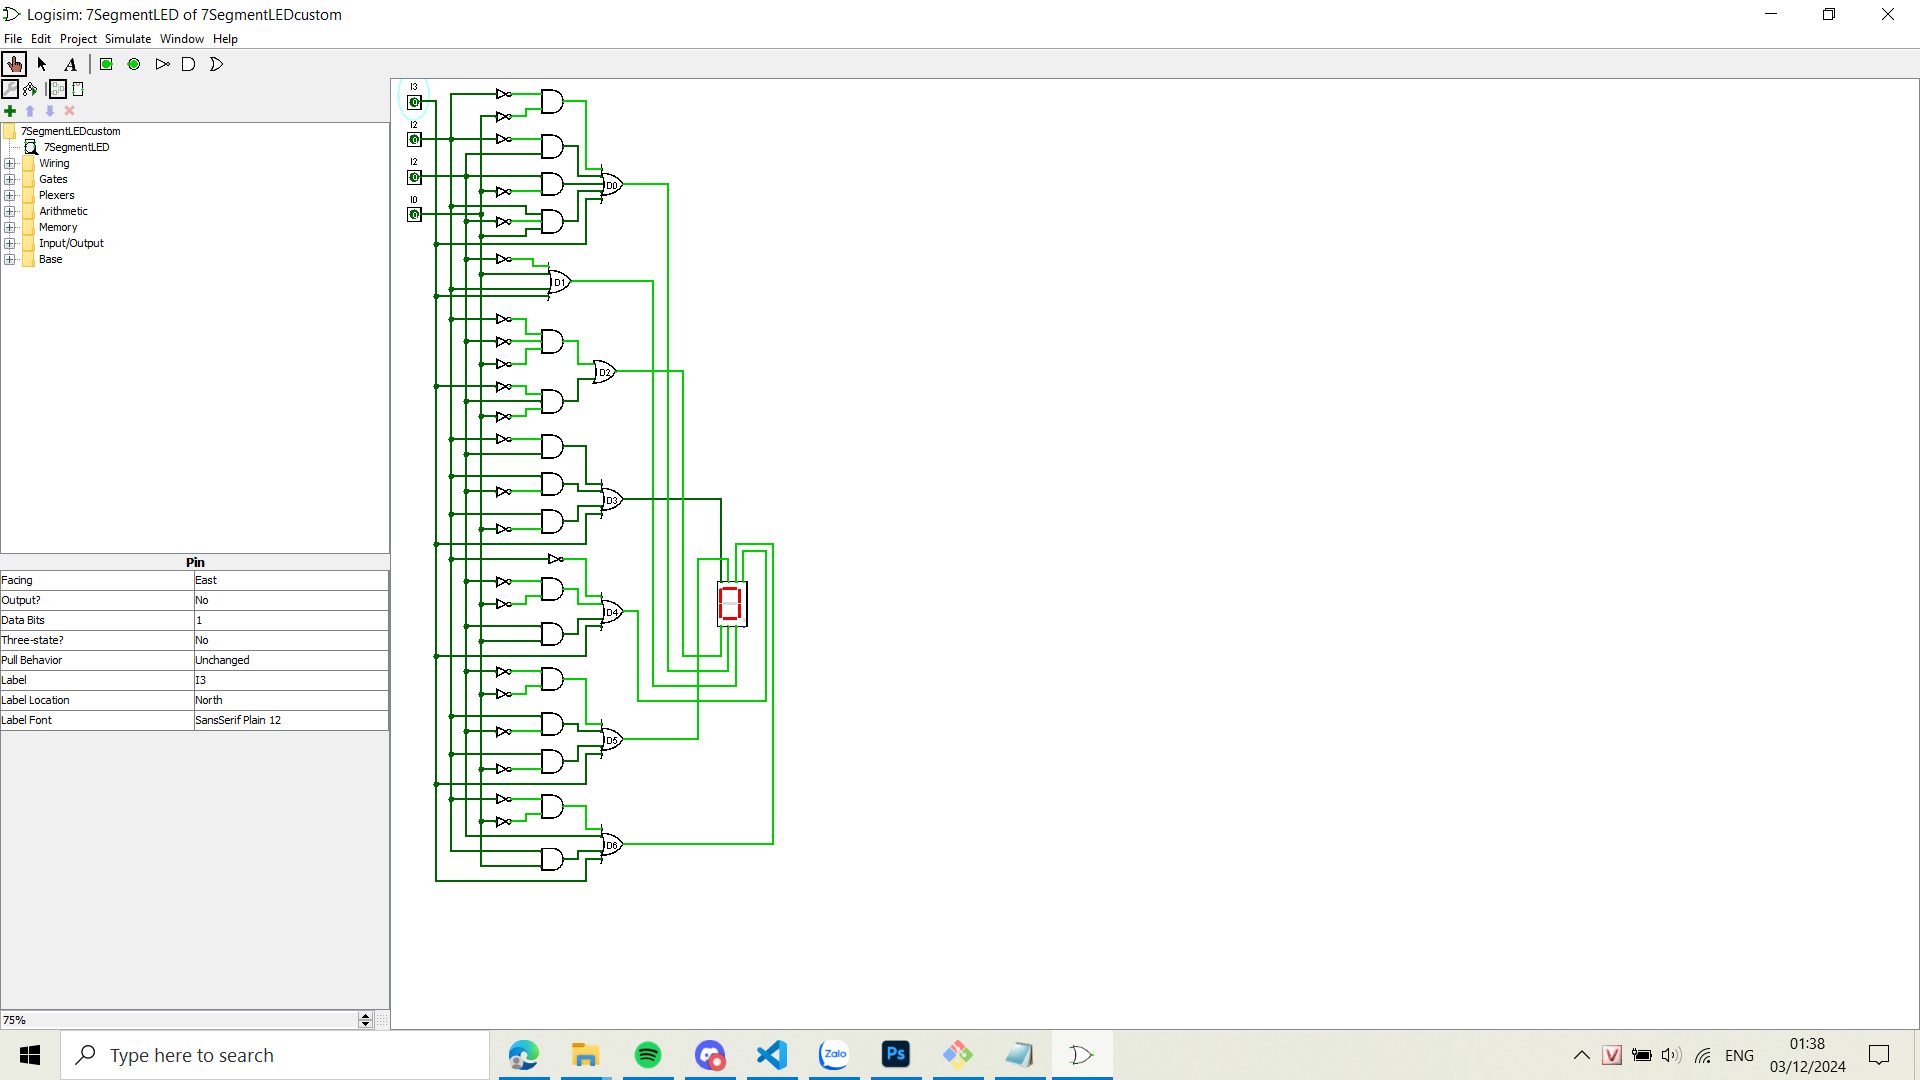
\includegraphics[width=0.8\textwidth]{images/0.PNG}
	\caption{Sơ đồ mạch thử nghiệm trên Logisim đang hiển thị số 0}
	\label{fig:circuitDesign}
\end{figure}

\begin{figure}[H]
	\centering
	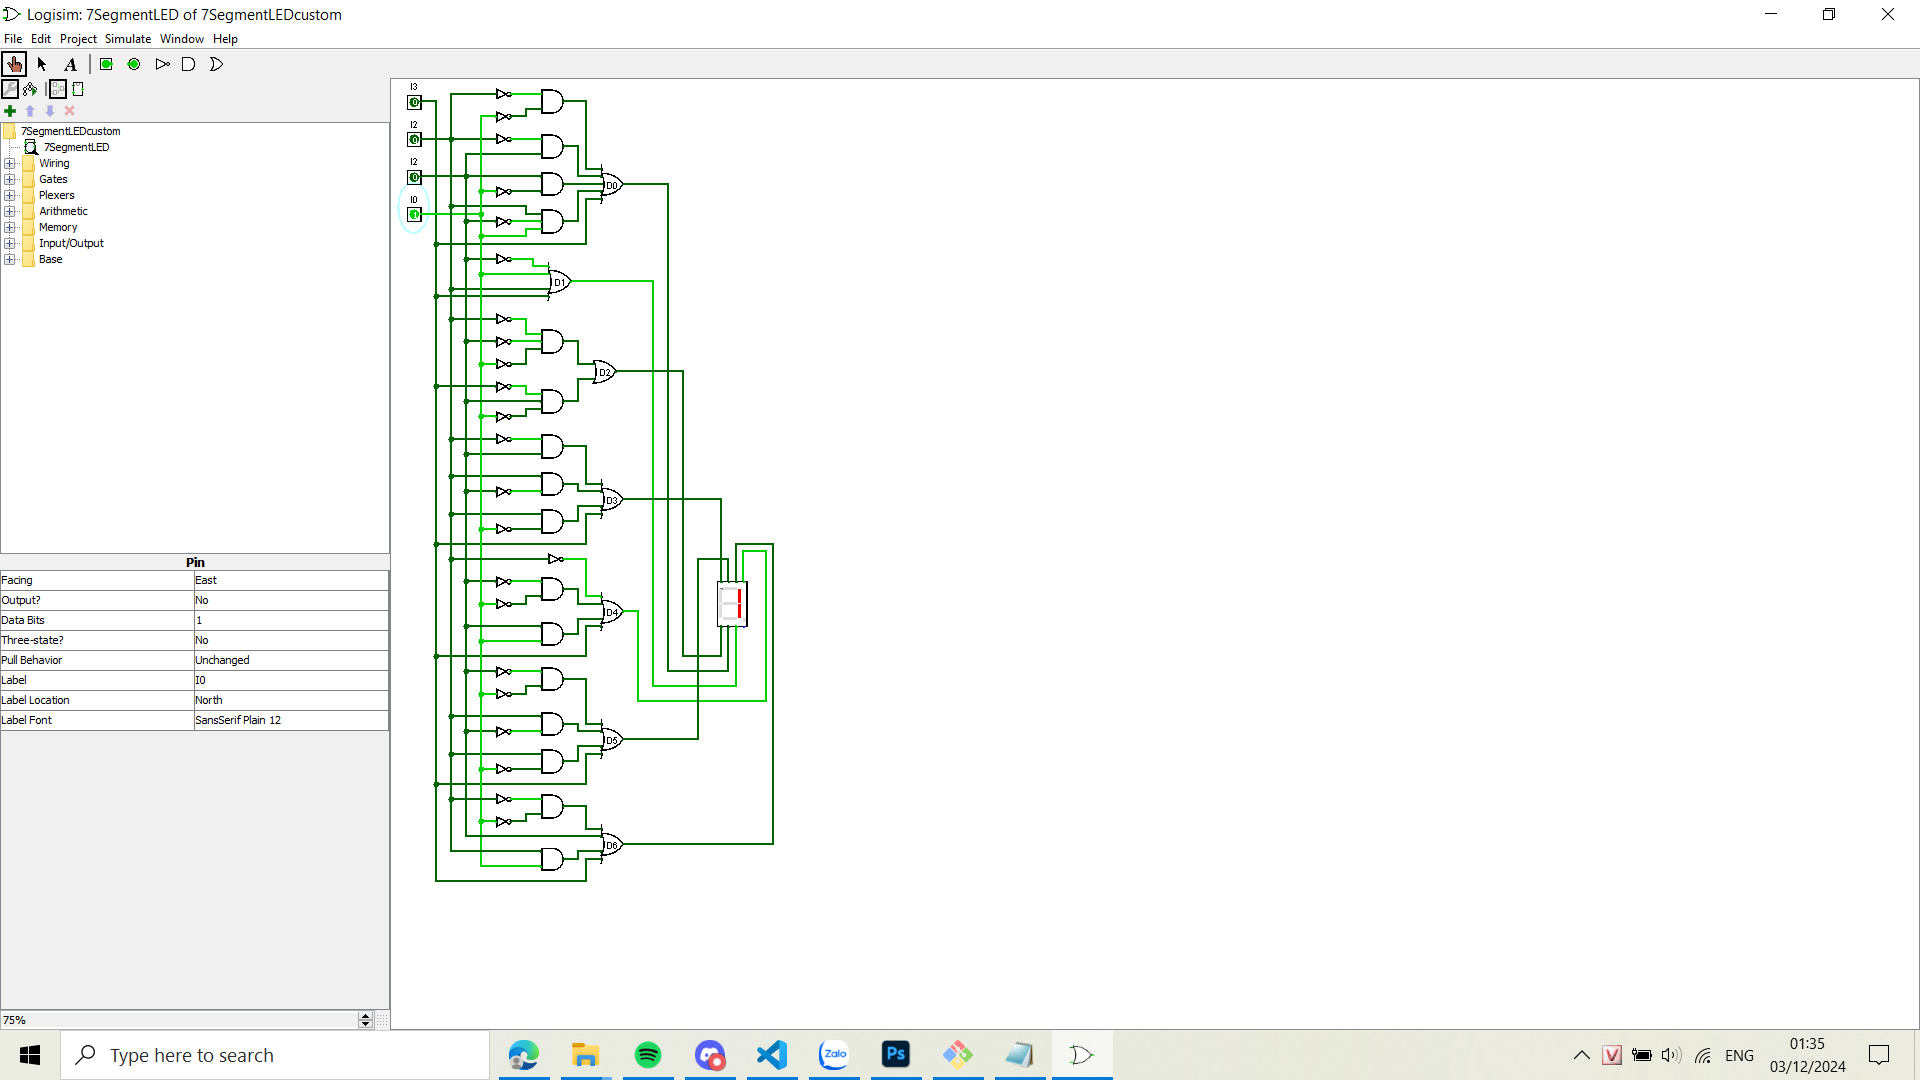
\includegraphics[width=0.8\textwidth]{images/1.PNG}
	\caption{Sơ đồ mạch thử nghiệm trên Logisim đang hiển thị số 1}
	\label{fig:circuitDesign}
\end{figure}

\begin{figure}[H]
	\centering
	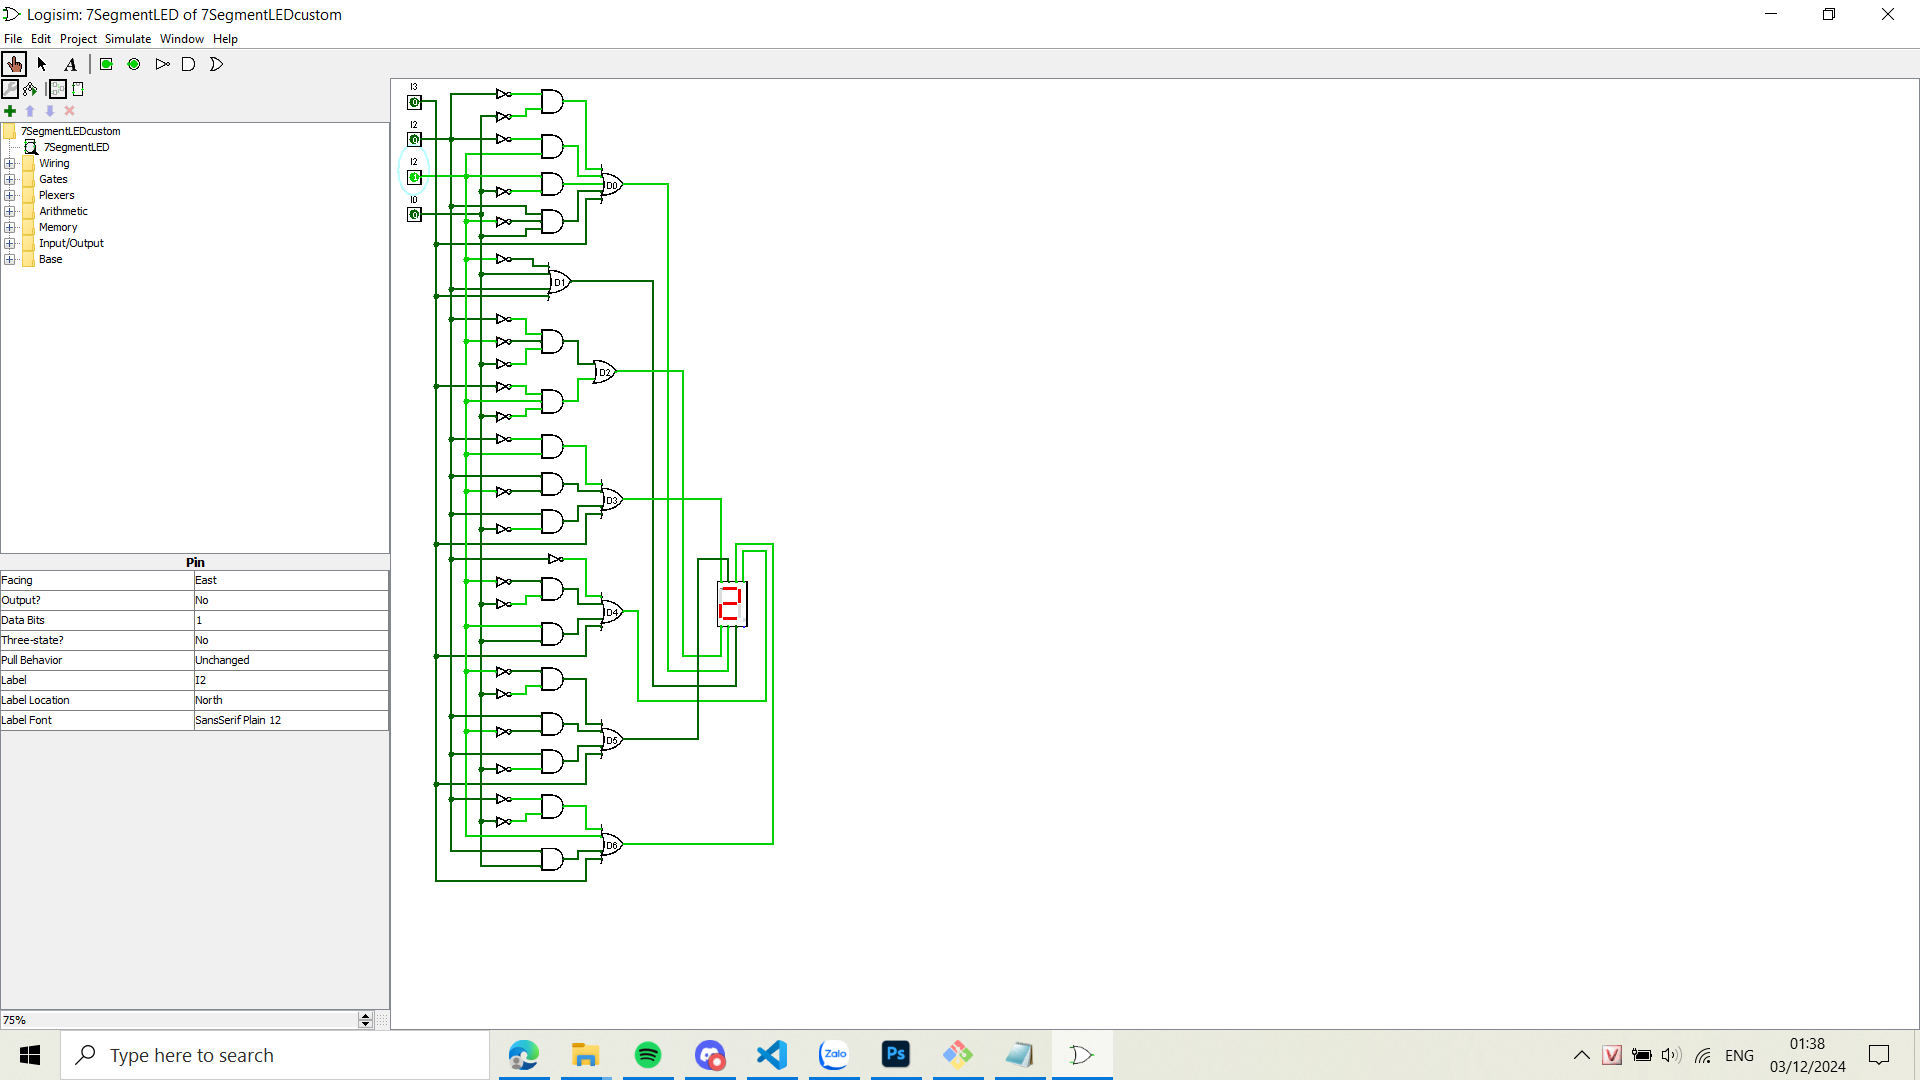
\includegraphics[width=0.8\textwidth]{images/2.PNG}
	\caption{Sơ đồ mạch thử nghiệm trên Logisim đang hiển thị số 2}
	\label{fig:circuitDesign}
\end{figure}

\begin{figure}[H]
	\centering
	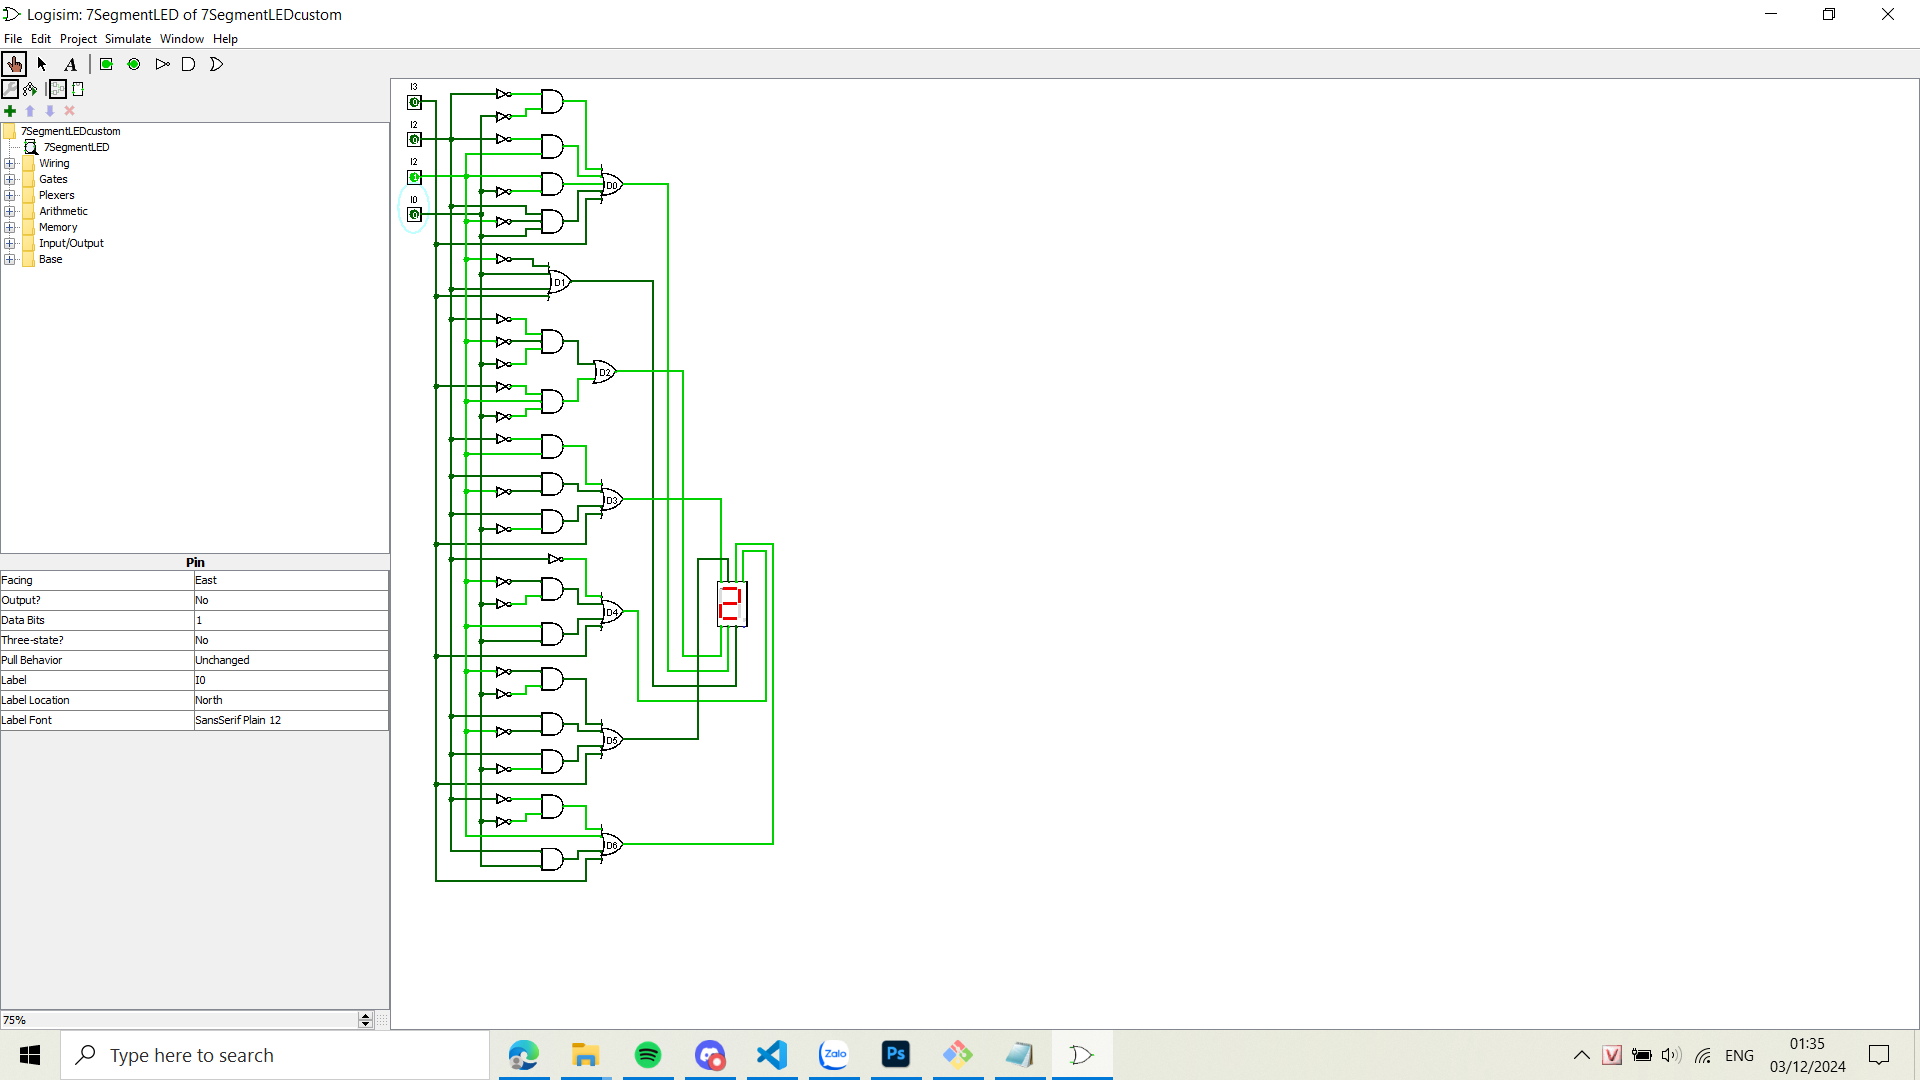
\includegraphics[width=0.8\textwidth]{images/3.PNG}
	\caption{Sơ đồ mạch thử nghiệm trên Logisim đang hiển thị số 3}
	\label{fig:circuitDesign}
\end{figure}

\begin{figure}[H]
	\centering
	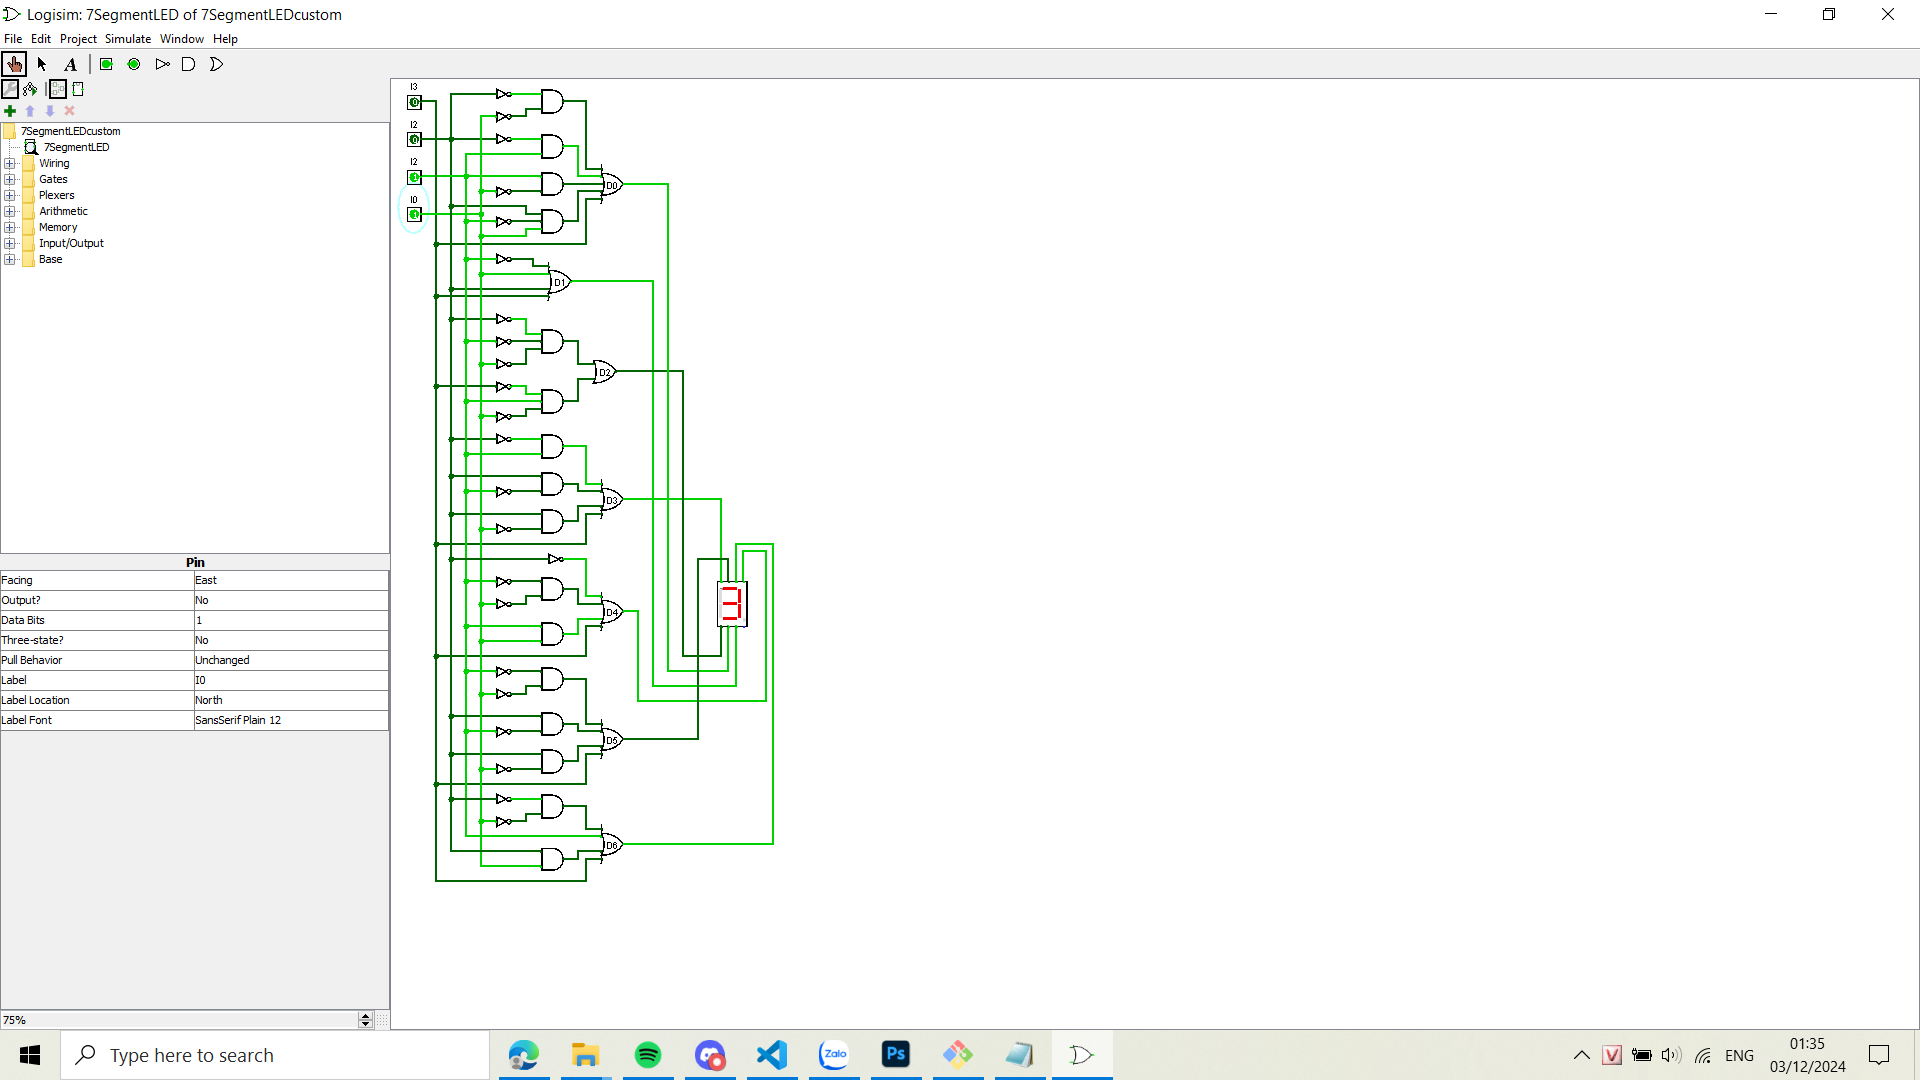
\includegraphics[width=0.8\textwidth]{images/4.PNG}
	\caption{Sơ đồ mạch thử nghiệm trên Logisim đang hiển thị số 4}
	\label{fig:circuitDesign}
\end{figure}

\begin{figure}[H]
	\centering
	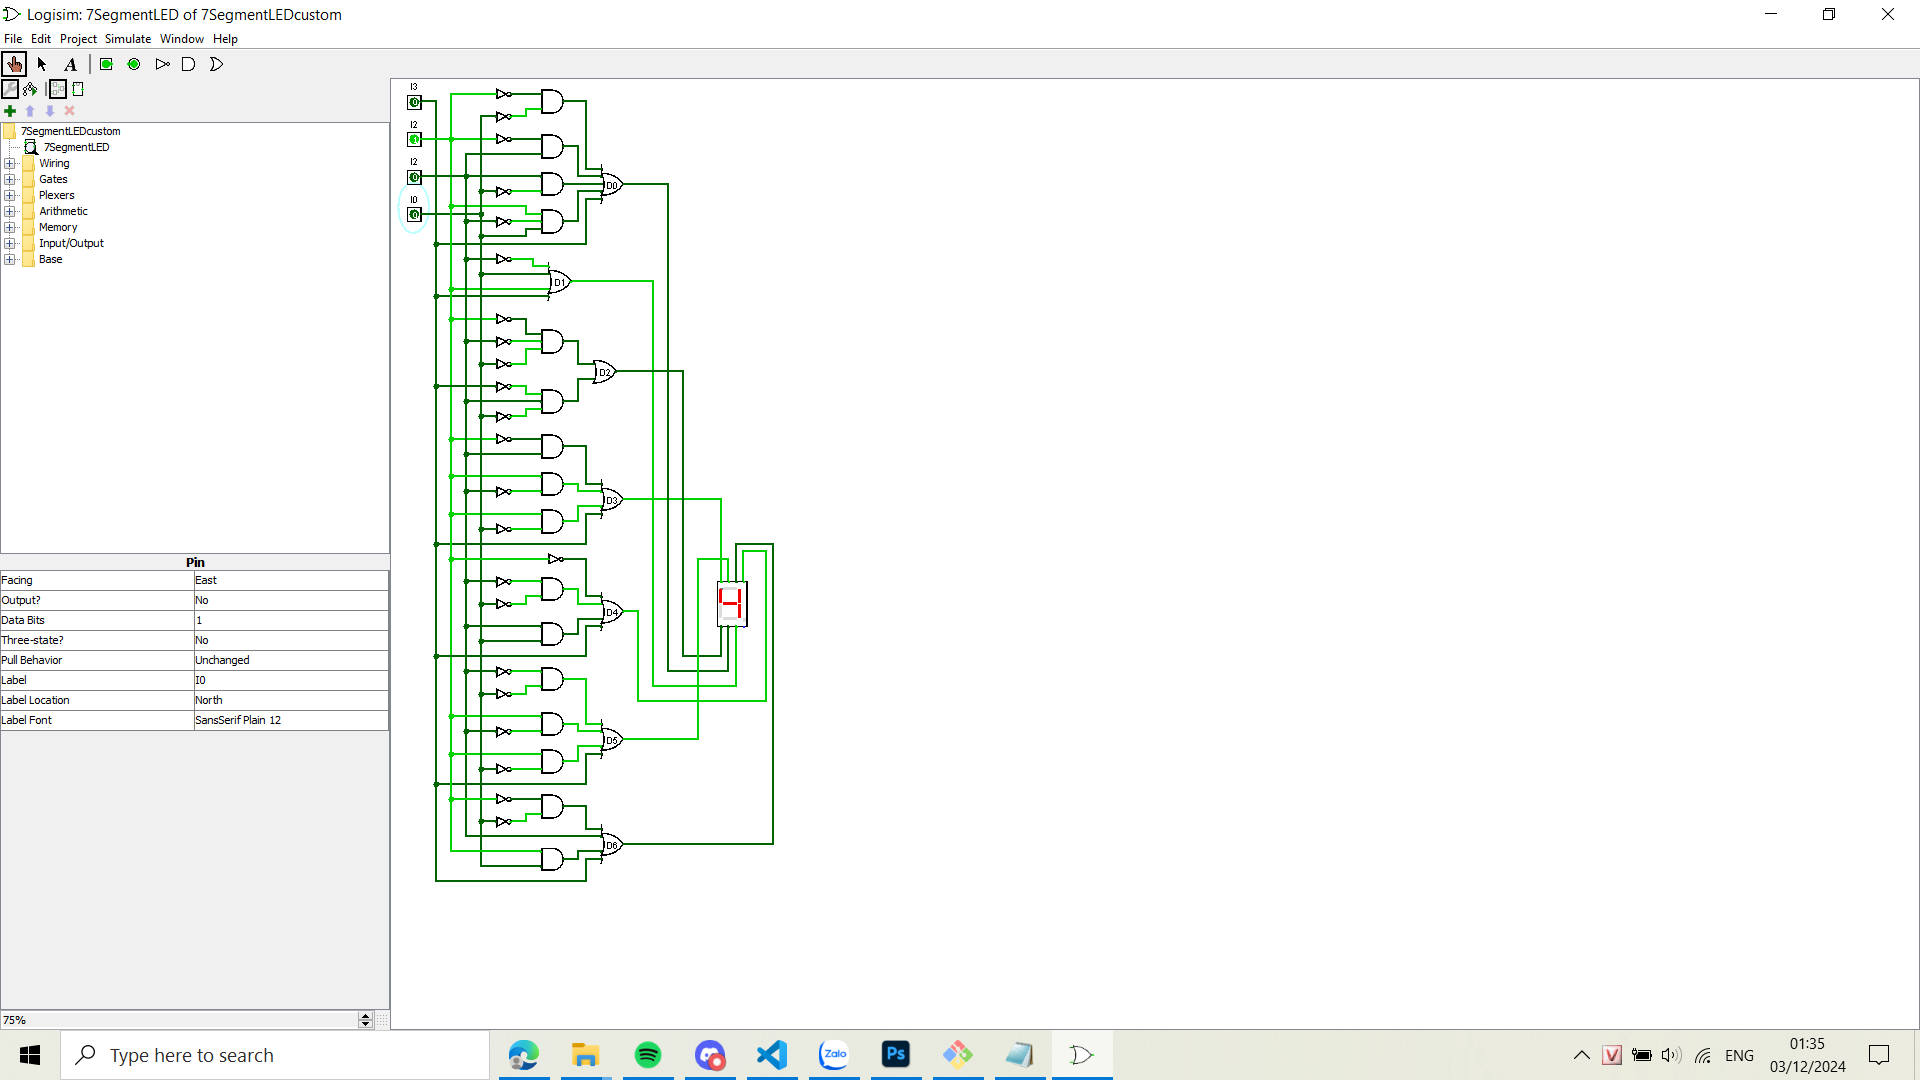
\includegraphics[width=0.8\textwidth]{images/5.PNG}
	\caption{Sơ đồ mạch thử nghiệm trên Logisim đang hiển thị số 5}
	\label{fig:circuitDesign}
\end{figure}

\begin{figure}[H]
	\centering
	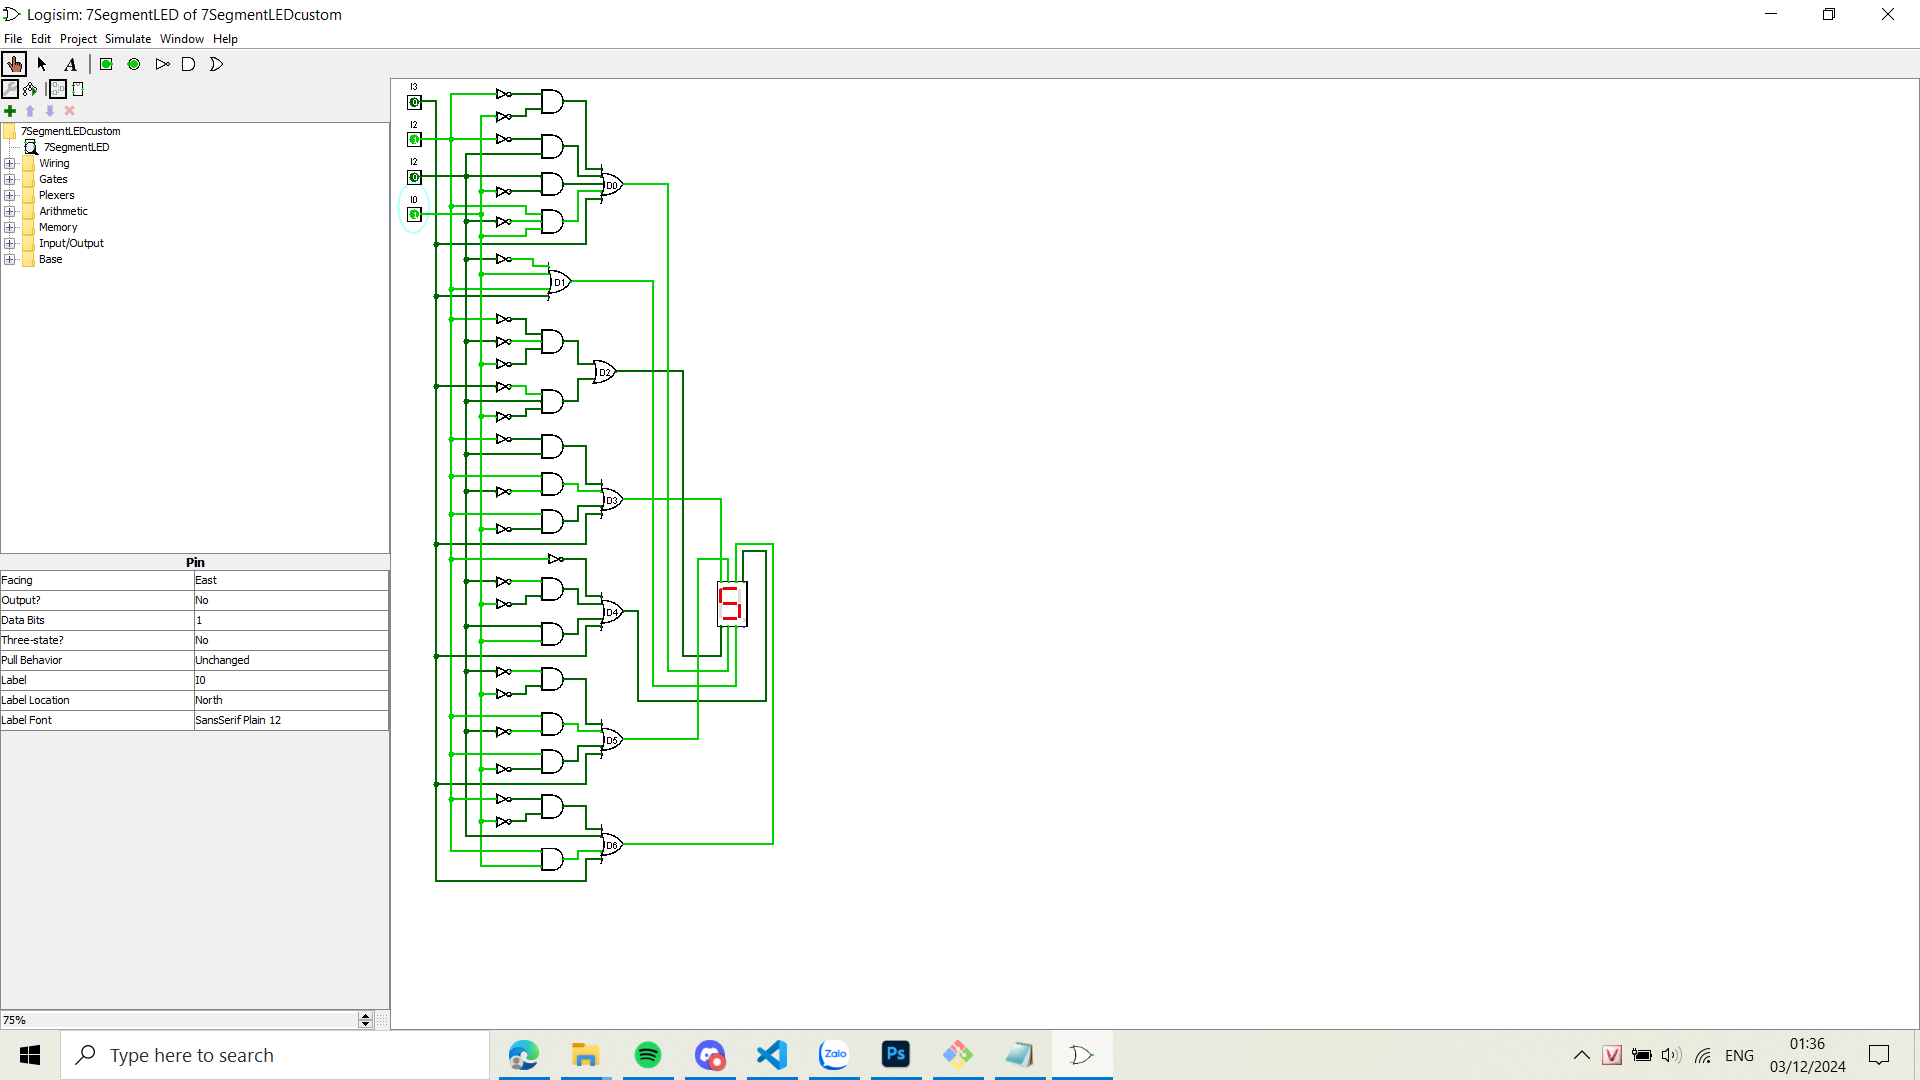
\includegraphics[width=0.8\textwidth]{images/6.PNG}
	\caption{Sơ đồ mạch thử nghiệm trên Logisim đang hiển thị số 6}
	\label{fig:circuitDesign}
\end{figure}

\begin{figure}[H]
	\centering
	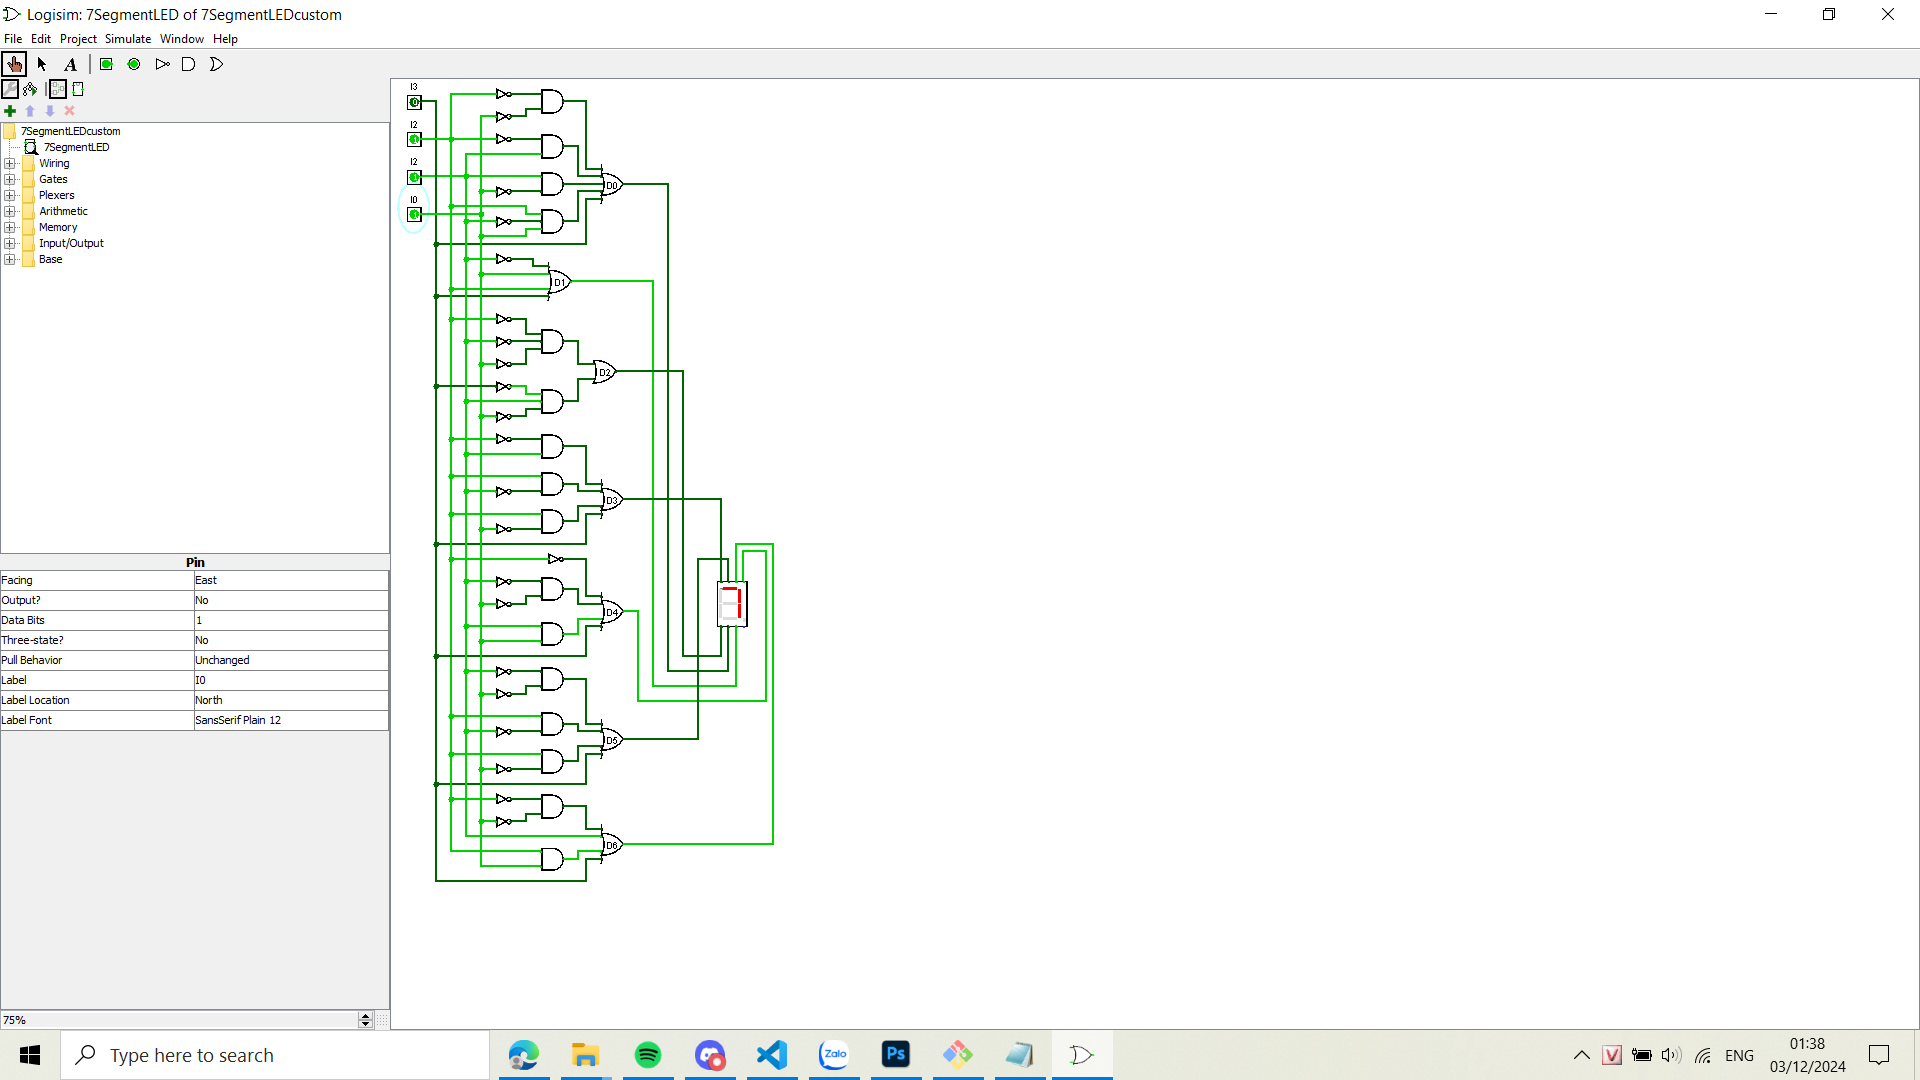
\includegraphics[width=0.8\textwidth]{images/7.PNG}
	\caption{Sơ đồ mạch thử nghiệm trên Logisim đang hiển thị số 7}
	\label{fig:circuitDesign}
\end{figure}

\begin{figure}[H]
	\centering
	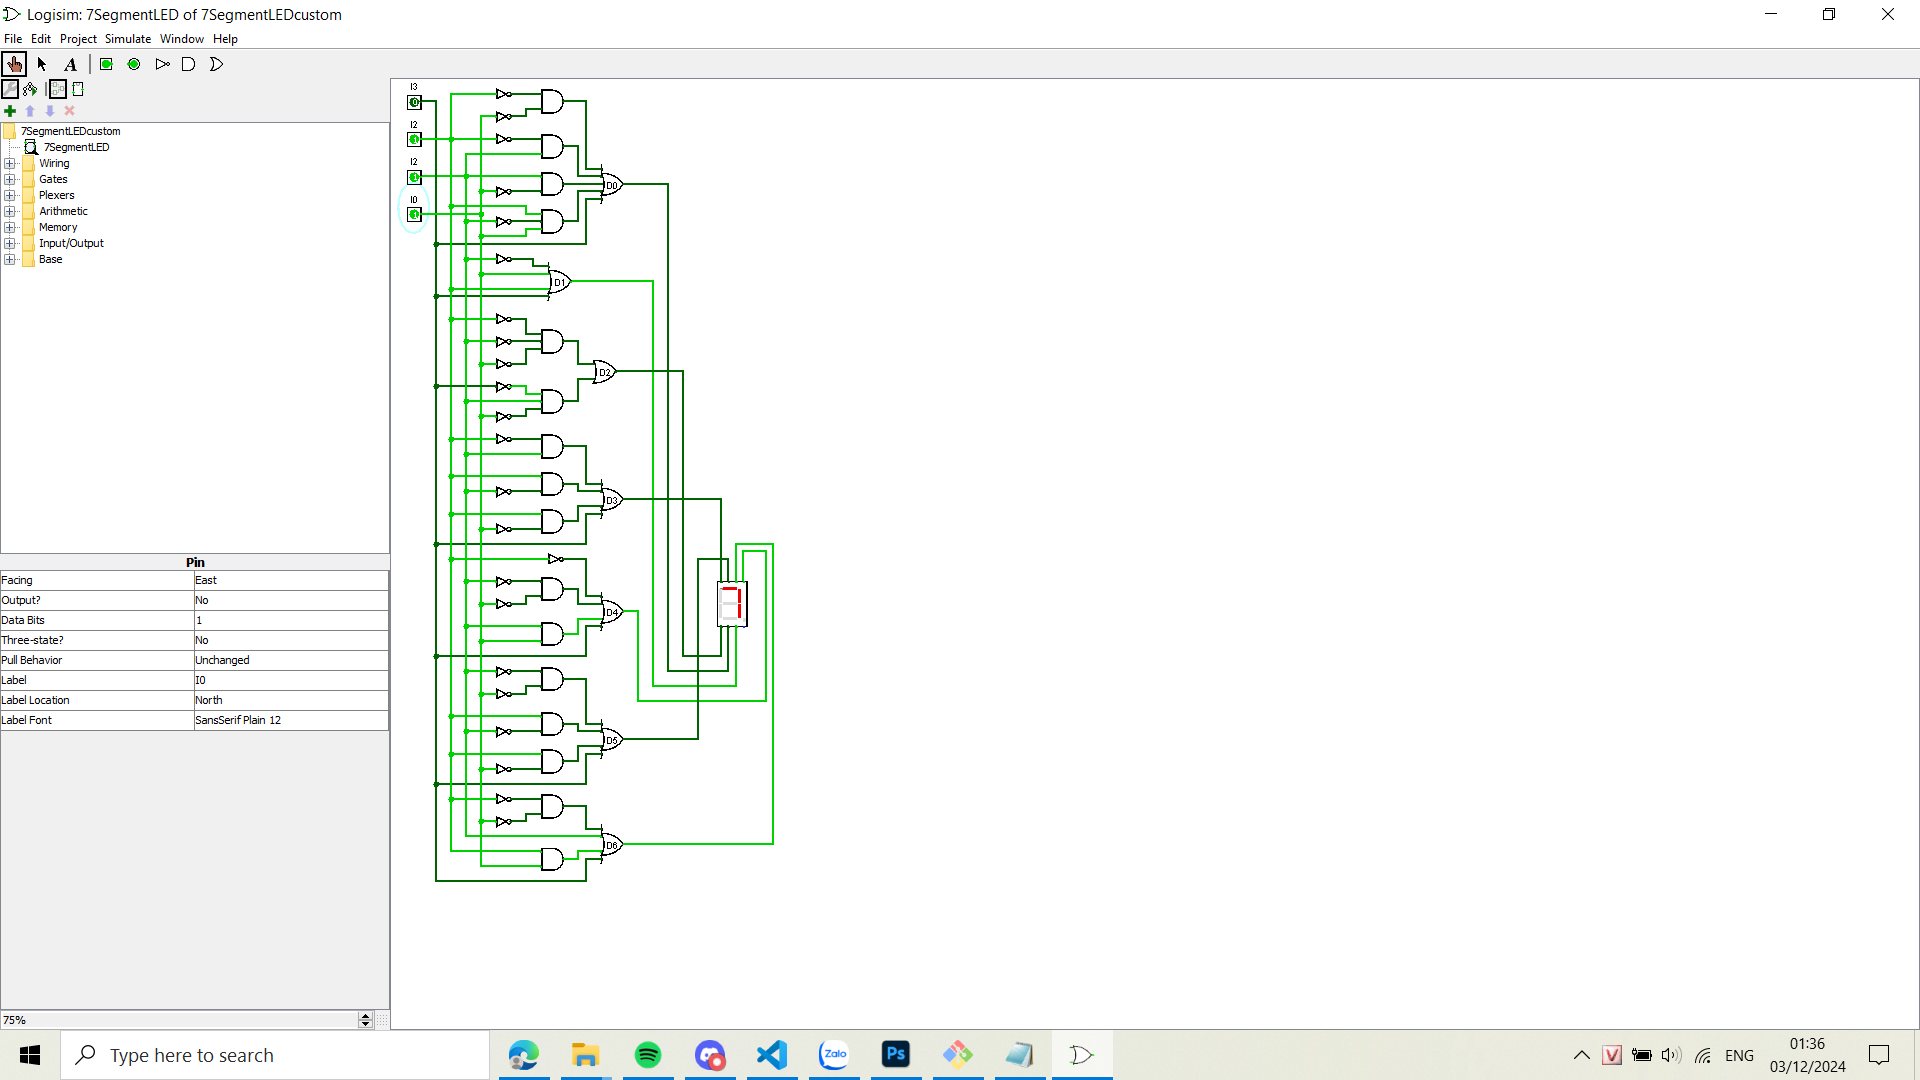
\includegraphics[width=0.8\textwidth]{images/8.PNG}
	\caption{Sơ đồ mạch thử nghiệm trên Logisim đang hiển thị số 8}
	\label{fig:circuitDesign}
\end{figure}

\begin{figure}[H]
	\centering
	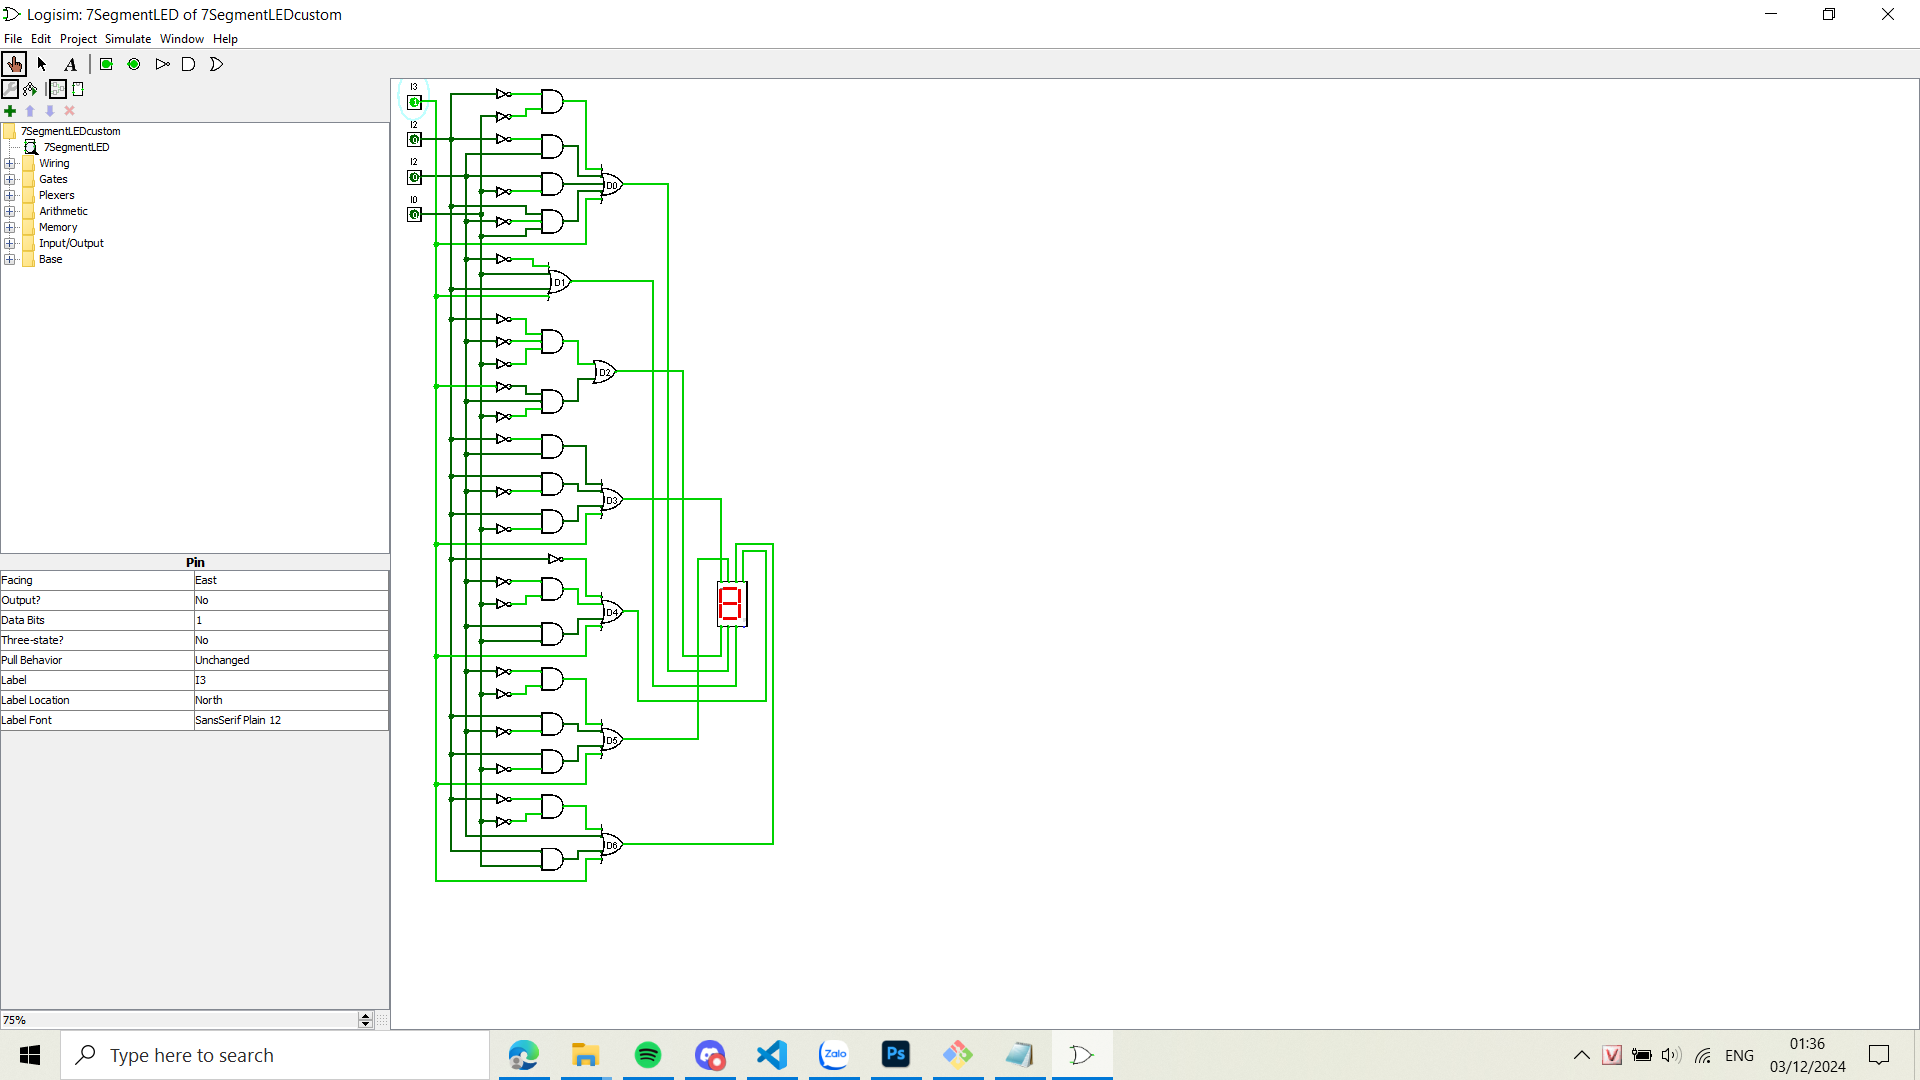
\includegraphics[width=0.8\textwidth]{images/9.PNG}
	\caption{Sơ đồ mạch thử nghiệm trên Logisim đang hiển thị số 9}
	\label{fig:circuitDesign}
\end{figure}

\section{Kết luận}

Sau khi hoàn thành bài tập này, em đã nắm vững kiến thức về cách thiết kế mạch LED 7 đoạn trên Logisim. Em đã hiểu cách kết nối các đoạn LED với các bit đầu vào và đã vẽ được sơ đồ mạch thử nghiệm trên Logisim. Bài tập này giúp em nắm vững kiến thức về mạch LED 7 đoạn và cách thiết kế mạch trên Logisim.

\section{Đánh giá}

\subsection{Bảng tự đánh giá các yêu cầu đã hoàn thành}

\begin{center}
	\begin{table}[H]
		\centering
		\caption{Bảng tự đánh giá}
		\renewcommand{\arraystretch}{1.4}
		\begin{tabular}{|l|p{\dimexpr0.6\linewidth-2\tabcolsep}|c|}
			\hline
			\textbf{STT} & \textbf{Yêu cầu}                                & \textbf{Mức độ hoàn thành} \\ \hline
			1            & Lập bảng chân trị với 4 bit đầu vào và 7 đầu ra & 100\%                      \\ \hline
			2            & Viết hàm luận lý cho mạch đèn LED 7 đoạn        & 100\%                      \\ \hline
			3            & Vẽ sơ đồ mạch thử nghiệm trên Logisim           & 100\%                      \\ \hline

			             & \textbf{Tổng cộng}                              & \textbf{100\%}             \\ \hline
		\end{tabular}
		\label{tab:mytable}
	\end{table}
\end{center}

\subsection{Nhận xét}

Bài tập đã hoàn thành đầy đủ các yêu cầu đề ra. Tất cả các bước đều được trình bày rõ ràng và chi tiết. Tổng thể, bài tập đã hoàn thành 100\% các yêu cầu đề ra.